\chapter{Introduction}\label{ch:introduction}
\setlength{\epigraphwidth}{3in}
\epigraph{Three can keep a secret, if two of them are dead.}{Benjamin
  Franklin}

This book is about finding and exposing data that are \emph{hidden}, \emph{invisible}, or simply
easy to \emph{overlook} in digital systems. Such data, when present
without our knowledge, can damage privacy, cause pain, ruin
reputations, cause financial loss, or even harm national security. The
purpose of this book is to teach you methods for finding and exposing
these data leaks so that you can prevent them from happening in the
future.

Secrets are present in many computer systems. They are stored in
documents, embedded in operating systems, and even sent over
information networks. It's not the presence of the secrets that
damages privacy---it's the release of documents or data that are
thought to be clean, but actually contain hidden information that
should have been kept private. 

Consider these two cases:

\begin{itemize}
\item In April 2011, the UK Parliament posted an Adobe Acrobat Portable
Document Format (PDF) file on its public website detailing key
vulnerabilities of UK nuclear subs. The electronic document had been
cleared by the British Ministry of Defense, where an official had been
charged with removing the sensitive portions, but the redactions were
made incorrectly: the sensitive text had simply been obscured with a
black box, and could be recovered by copying the text out of the PDF
file and pasting it into a word processor. The result was a document
that appeared to be properly redacted, but which still contained state
secrets.  A follow-up investigation by \emph{The Daily Telegraph}
found similar PDF files in which sensitive information was improperly
``redacted'' on four other UK government
websites\cite{telegraph-april2011-secrets}.

\item Also in April 2011, two security researchers discovered that
Apple's iOS~4 operating system was tracking the movements of every
iPhone and iPad and storing that information in a database on the
mobile device. This database was copied to the users'
desktop or laptop computer whenever they backed up their mobile
device. The researchers, Pete Warden and Alasdair Allan, discovered
the file by accident---but they understood its
importance\cite{apple-tracking}. Warden and Allan developed an application that
took the data and plotted it on a map, with larger dots indicating
more data points~(\figref{heatmap}). A media uproar resulted, and
Apple released a new version of iOS that fixed the bug shortly
thereafter\cite{apple-tracking-statement}. 

\end{itemize}


\begin{figure}
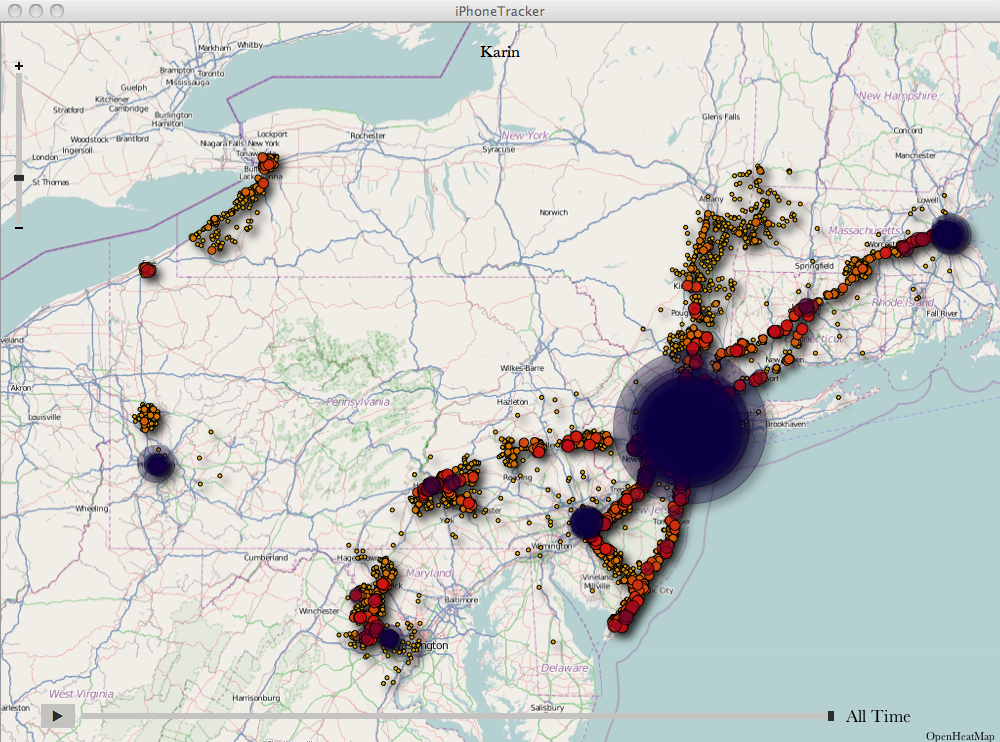
\includegraphics[width=\textwidth]{ch-1/5637893141_ba59f2d989_o.png}
\caption{In April 2011 two researchers discovered that Apple's iOS 4
  operating system recorded the location of nearby Wi-Fi access points
  to aid in geolocation. Due to a bug the database was never
  cleared. As a result, the database could easily be used to create a
  map of every place that the iPhone had been. (C) 2011 John
  Niedermeyer. {\small (Licensed under Creative Commons
  Attribution-NonCommercial-ShareAlike 2.0 Generic)}}\label{heatmap}
% http://www.flickr.com/photos/nedward/5637893141
\end{figure}

Over the years a wide variety of software running on many different
kinds of computers have been responsible for significant privacy and
security violations. The violations are typically
\emph{unintentional}---the people who wrote these programs didn't
create them with the goal of violating privacy. Instead, the programs
have had bugs or usability flaws that caused private information to be
inadvertently retained or distributed. The software problems are
typically so subtle that most users don't realize that their private
information is being compromised. And because the private information
leaked is typically embedded in a form that is invisible or easily
ignored, the flaws can persist for weeks, months, or even years before
they are discovered and fixed.

Inadvertent privacy leaks aren't limited to government agencies and
major computer manufacturers: many damaging privacy leaks happen
person-to-person because modern computer systems are so
complex. Consider the digital photograph shown in \figref{nsf_hq}. The
original photo was 3264x2448 pixels and clearly showed a readily
identifiable 12-story office building. The cropped version is 1248x699
and does not contain much identifying information. But the cropped
version still contains the metadata from the original; this metadata
describes the time that the photograph was taken, the fact that it was
taken with an iPhone 4S, and the GPS location of the
photographer to within a few feet. (\figref{nsf_metadata}). 

It turns out that there are several different ways to crop JPEG
photographs on the Macintosh computer that was used to make
\figref{ch-1/nsf_hq}. One of the programs is Apple's iPhoto, which has
check boxes for including ``Title and keywords'' and ``Location
information'' on its export dialog box. 

\sgraphic{ch-1/nsf_hq}{This photograph of a tree and a few cars contains
  and embedded title and GPS location information.}

\bifigure{ch-1/nsf_hq_exif}{ch-1/nsf_hq_gps}{Metadata from \figref{ch-1/nsf_hq}, as displayed by the Apple
  Macintosh Preview application.}

\bifigure{ch-1/export}{ch-1/export1}{Apple's iPhoto (left) allows the user to select whether or not
  titles and location metadata will be included in exported
  photographs; Apple's Preview tool (right) copies metadata without
  warning the user.}

\section{Technical Privacy Auditing}

This book teaches some of  ways that private information has been
leaked in modern information systems and shows how you can find 
those leaks using tools that are freely available. We call this
process ``technical privacy auditing'' because it uses technical
tools to find privacy problems in software.

Most of the technical privacy failures that we know about were not
discovered by the companies that wrote the software in
question. Instead, they were discovered by students,
journalists, and computer enthusiasts---people who looked at the data
and saw something that they thought was worth investigating.

The root cause of many technical privacy violations is the complexity
of modern information systems. Today's computers are vast, with
gigabytes of storage, tens of thousands of application programs, and
real-time connections to data networks that continually download ever 
more code and data. A typical cell phone with 16 gigabytes of memory can
store literally hundreds of thousands of digital photographs, hours of
video, or months of audio recorded from its internal
microphone. It's very easy for a programmer to overlook some small
piece of storage that may hold some very sensitive piece of
information. 

The basic premise of this book is that many such privacy leaks can be
discovered through straightforward visual inspection---provided that
you know where to look---and they can frequently be avoided with
relatively simple software modifications. Our goal is to teach you flexible, general
purpose approaches for finding that data and clearly documenting the
problem for others. This
will put you in the position to discover new privacy and security
leaks in the future and for getting them fixed.

Privacy leaks such as the hidden information in PDFs and Apple's
unintentional location database are insidious because they are
invisible. They can be present for years in a piece of software that's
used by millions of people. They can be exploited against the interest
of their users. And they are frequently present because nobody looked
deeply at the data or publicized their findings. 

\section{Digital Forensics Tools}

This book teaches approaches for finding leaks of personal information using
digital forensics tools. The previous section gave a brief description
of two kinds of leaks that have happened in recent years. This
section gives a brief introduction to digital forensics, the digital
forensics process (called the ``model'' by practitioners), and how the
leaks described in the first section could have been found using
digital forensics tools.

\subsection{Digital Forensics}

\emph{Digital Forensics} (DF) is a branch of forensic sciences that
involves the investigation digital devices and the data that they
contain for the purpose of proving or disproving a hypothesis about an
event that took place in the past. For example, digital forensics
tools can be used to extract a deleted photograph from a cell phone
and present that photograph in a court of law. The forensic process
can be used to determine whether or not the photograph was taken by the
phone's camera or downloaded to the phone over a network. The process
can also be used to establish when and where the photo was taken.

In recent years the rise of television forensic shows like CSI and
NCIS have presented a somewhat distorted view of DF to
the general public. While the shows accurately convey the important
role that DF has in some cases, television forensics departs from
reality in many important ways. 

On television, forensics is portrayed as being swift and
certain. Forensics software is graphical, easy-to-use, and fast. For
dramatic reasons the forensics team typically has just one or two
specialists that know how to perform a forensics analysis, and they know how
to use \emph{every} tool that the organization has---digital tools,
fingerprints, chemistry, and even nuclear physics. There are typically
no false positives or mismatches in televised forensics. Data that are
overwritten or encrypted can usually be recovered (unless the plot
requires that they not be), and it is nearly impossible to delete
anything. Sadly, such portrayals have caused victims and  juries alike
to have unrealistic expectations about the technical capabilities of
government agencies, something that has come to be known as \emph{the
  CSI Effect}\cite{csi-effect}\cite{beyond-csi-effect}.

Privacy in the digital world would be at considerable risk if digital
forensics truly had such powers: anyone who desired could violate any
secret anywhere. Fortunately, the reality of digital forensics is far
less exciting---and decidedly more pro-privacy.

In the real world, data that are overwritten generally cannot be
recovered, and data that are encrypted usually cannot be
decrypted. This is good news from a privacy perspective: it means that
technical measured, properly applied, really can protect computer
users from accidental data leaks. 

From its inception, DF has served two different purposes:

\begin{enumerate}
\item \textbf{Extracting information from physical devices related to
  a crime.} In the pre-digital age a suspect's address book or
calendar might be entered directly into evidence and handed to the
jury. That's not possible in the digital age, when those materials
might be on a password-protected computer or hidden somewhere inside a
mobile phone. In many cases forensic techniques make it possible to
recover data that have been deleted or hidden but not yet
overwritten. 

\item \textbf{Understanding the details of crimes that are inherently
  digital (``cyber crime'').} DF tools allow the examination of
data from crimes that have no analog in the pre-digital world, such as
breaking in to a computer over a network or planting malware on a
person's mobile phone. In these kinds of cases, DF tools may be the
only way to understand what has happened and attempt to determine the
responsible party. 

\end{enumerate}

DF is powerful because computer systems are windows into the
past. Many digital systems retain vast quantities of
information---either intentionally, in the form of log files and
archives, or inadvertently, as a result of software that does not
cleanly erase memory and files after it runs. As a result, it
is frequently possible for investigators to recover old email
messages, chat logs, Google search terms and other kinds of data
that were created
weeks, months, or even years in the past. Such contemporaneous records
can reveal an individual's state-of-mind or intent \emph{at the time
  the crime was being committed}.

The next section describes how digital forensic tools can be used to
accomplish these goals.

\subsection{The Digital Forensics Model}

Even though every case is different, DF practitioners have developed an
approach to conducting investigations called the 
\emph{digital forensics model}\cite{pollitt:models}. The 
elements of the model include:

\begin{description}
\item[Preparation] Before performing an investigation, those involved
  must prepare themselves by deciding upon the standards and
  procedures that will be followed; receiving the necessary training;
  and obtaining the appropriate equipment and software required for
  investigations. 

  To use the example of the cell phone from above,
  preparation may involve obtaining specialized hardware that can extract the
  memory from a cell phone and practicing one's technique on phones that are not part
  of the investigation.

\item[Collection and Preservation]
  Before data can be analyzed, they   must be removed from the
  device being analyzed and preserved to create a lasting
  record. Without this step, it may not be possible to repeat an
  analysis at a later point in time. 

  In our example, this step might involve the actual extraction of data
  from the cell phone into a single file called a \emph{physical
    image} that records all of the phone's applications, phone data, user data,
  and deleted files. Such a physical image might be 64GB in size or
  even larger.

\item[Examination and Extraction] Working with the preserved data, an
  examiner will explore for any information that might be
  relevant to the investigation at hand. Once that information is
  found, it is extracted and isolated.

  In our example, this step might involve the extraction of each
  digital photograph from the \emph{physical image} and the storage of
  each photograph in its own file. The files might be named according
  to where they were found in the physical image (e.g. 62071808.jpg)
  rather than with the name that they were given by the phone
  (e.g. IMG001.JPG). The examiner might also extract \emph{metadata}
  from each photograph such as the time and GPS coordinates associated
  with each exposure and the serial number of the camera that took the
  photograph. This information might be stored in a separate file for
  each photograph (e.g. 62071808.txt) or might be stored in a single
  spreadsheet for all of the photographs (e.g. jpeg-metadata.xls).

\item[Analysis] Once the specific data being analyzed has been
  extracted, the analyst will construct one or more hypotheses that
  uses the digital evidence to explain possible past activities. A
  hypothesis may draw from multiple digital devices---an email message
  sent from a desktop computer to a cell phone, for example---or the
  hypothesis may incorporate events in the physical world, like a
  power failure or theft. During this phase a good analyst will also
  try to construct alternative hypotheses that are consistent with the
  evidence but which point to different conclusions. 

  In our example, the hypothesis may be that a specific photograph was
  taken with the phone in question. This may be supported by the
  photograph having similar metadata to a photograph taken a few
  minutes earlier or later. An alternative hypothesis may be that the
  photograph was downloaded to the phone over a network.

\item[Reporting and Testimony] Finally, the analyst will
  produce a written report or give testimony in a courtroom.
  Judges and juries can't examine digital evidence for
  themselves---even if they had the training and the technical skills
  to do so, performing their own analysis would be inappropriate:
  their role in the legal process is to evaluate the law, the evidence
  and make a legal determination, not to perform technical
  analysis. Reports and testimony must therefore be 
  \emph{complete}---they must describe the tools and procedures
  that were followed, clearly document what was found, and then
  separately provide the technical interpretation of the
  evidence. 

  In our example, the analyst might prepare a report documenting how
  the phone's contents were copied, the tools that were used to
  extract the photographs and their corresponding metadata, and how
  the evidence is consistent with the analyst's hypothesis. 

\end{description}

The model brings reliability and repeatability to the process, helping
to assure that different examiners working with the same data will
arrive at the same conclusion. 

Because they can look into the past and uncover hidden data, DF tools
are increasingly used beyond the courtroom. Security professionals use
DF tools to analyze network intrusions---not to convict the attacker,
but to understand how the attacker gained access to plug the
hole. Data recovery firms use DF tools to resurrect files from drives
that have been inadvertently formatted or damaged. 

\subsection{A Microscope for finding Personally Identifiable Information (PII) }

Our goal is to use
the model for privacy auditing. We want to detect the presence of
information that is personally identifying or potentially
sensitive. To do this, we'll use DF tools as a kind of digital
microscope. Like a biologist looking for bacteria or other signs of
contamination, if we find sensitive information, we'll know that there is a potential
for a privacy leak.

The term \emph{personally identifiable
  information} (PII) is frequently used as shorthand sensitive
information that should not be disclosed, and we'll use that shorthand
here. The term is unfortunate, however, as not all personally identifiable information is
sensitive and not all sensitive information leaks personally
identifiable information. Nevertheless the term is widely used and
even enshrined in many US laws, so we will use it here as well.

Our basic approach will be to treat privacy auditing as an
experimental science. We will create specially manufactured documents,
computer media and network streams that are likely to contain known
PII. We will then use DF tools to see if we can find the PII that we
have inserted. This will allow us to both understand how the tools
work and how the PII moves through a digital system. Finally, we will
apply the same tools to documents, media and network streams acquired
in the ``wild''---in the digital environment---and see if those wild
samples contain PII. If they do, we have documented a privacy failing.

Others have used DF tools for this purpose. For example, in 2009 the
Inspector General of the United States Department of Defense issued a
report in which forensic software was used to test hard drives leaving
the government service. The IG found that ``DOD Components did not
properly sanitize, document, or fully account for excess unclassified
IT equipment before it was released to other Federal, DOD, or
non-Federal organizations.''\cite{D-2009-104}

Both of the privacy leaking examples at the beginning of this chapter
could have been readily prevented by applying the digital forensics
model:

\begin{enumerate}
\item \textbf{The UK PDF files.} The reports in the British
  newspapers demonstrated  that it didn't take specially trained DF
  practitioners using expensive tools to recover the data from the
  MoD's improperly redacted PDF files. All that was required was a
  copy of Adobe Acrobat Reader. 

  Applying the DF model would have put the MoD in a better position to
  preventing the disclosure in the first place. Starting with proper
  training, the organization would have been better positioned to
  understand the difference between removing sensitive information and
  simply covering it up. After the files were sanitized, forensic tools
  could have been used to search for key words, terms,
  or labels associated with sensitive or restricted information: if
  such keywords were found, the tools could have been used to identify
  the process failings. When the redaction process was corrected and
  re-applied, the tools could then verify that the redaction had been
  completed as expected.

\item \textbf{The Apple Geolocation Database.} Likewise, Warden and Allan didn't
  require special forensic tools to find the covert geolocation
  database that was present in iOS~4. The database was a standard SQLite3
  file, and the file was stored as part of the iPhone ``backup''
  database present on every Macintosh or Windows computer that was
  synched with an iPhone using Apple's iTunes program. The database
  was ready to be found by any privacy professional that did an audit
  of those files, for the simple fact that it was larger that all of
  the other databases in the backup: whereas most of the databases were typically
  10KB to 100KB in size, the geolocation database from some iPhones was
  in the 10MB to 100MB range. The database was so large because it was
  never pruned; it was a privacy violation for the same rason.

  The computer forensics model applied to the iPhone system could have
  readily caught the privacy leak before the iPhone software was
  released to the general public. An important part of the Analysis
  step is to look for and try to explain outliers: the database
  was such an outlier that should have attracted attention. 
\end{enumerate}


\section{Conventions used in this book}
In general this book follows \emph{Wikipedia Manual of
  Style}\footnote{\url{http://en.wikipedia.org/wiki/Wikipedia:Manual_of_Style}}
and specifically the Computer
Science\footnote{\url{http://en.wikipedia.org/wiki/Wikipedia:WikiProject_Computer_science/Manual_of_style}}
  and
  Computing\footnote{\url{http://en.wikipedia.org/wiki/Wikipedia:Manual_of_Style/Computing}}
  sections. Specific conventions useful in understanding this book are
  described below.

\subsection{Fonts}

Text in this book is generally typeset in the serif font that you are
now reading. The fixed-width courier font is used for programs,
computer input and output, as well as for numbers that might
reasonably be expected to be constants in a computer program. Thus,
the Earth is 150 million kilometers (150 Gm) from the sun, but a
traditional disk sector has |512| bytes (|512|~B).

\subsection{Radix}
Numbers are generally assumed to be in base 10 unless otherwise
specified. Binary digits are suffixed with a |b|; octal
is indicated with a leading |0| as in most programming
languages; hexadecimal numbers may be prefixed with |0x| or |\x| or
have a |h| suffix. Unfortunately there are
exceptions that must be inferred from context. For example, hex dumps
and cryptographic hashes are always presented courier as unadorned hexadecimal
digits. Examples are shown in \tabref{nomenclature}.

\begin{table}
\begin{tabular}{cllrl}
     &              &         & Decimal  \\
Base & Nomenclature & Example & Equivalent      & Usage \\
\hline
\hline
2  & Binary      &  |10101111b|& 175            & Text\\
\hline
8  & Octal       &  |0377|     & 255            & Text and code\\
   &             &  |\377|     & 255            & Code\\
\hline
10 & Decimal     &  |1234|     & 1234           & Text and code\\
\hline
16 & Hexadecimal &  |DEADBEEFh|& 3,735,928,559  & text \\
   &             &  |0xFF|     & 255            & Output \\
   &             &  |\xFF|     & 255            & Python code\\
\hline
\hline
\end{tabular}
\caption{Examples of numbers in various bases used in this book.}\label{nomenclature}
\end{table}

\subsection{Units}

Measurements for Natural phenomena discussed in this book are provided
in SI Units (the ``Metric System.'')
Manufactured objects are described in either SI units or
United States customary units (followed by SI approximations), depending on the system of measurements
that was used to design and produce the object. Thus, this book
discusses 5.25-inch (133mm) floppy disks.

\subsection{SI and IEC Multipliers}\label{sec:si-and-iec}
% \note{1MB = 1,000,000 bytes}
% \note{1MiB = 1,048,576 bytes}

Today there are two standards in computing for representing sizes of
files, storage systems, and memory banks: SI (the International System
of Units) decimal prefixes and IEC (International Electrotechnical
Commission) binary prefixes. This situation is confusing because until
recently the SI prefix names \emph{kilo}, \emph{mega} and \emph{giga} were commonly used
for both decimal and binary notation, the specific multiplier presumably
inferred from context. Today there is an effort underway to clarify
usage. 

SI decimal prefixes are commonly used to represent SI
quantities. For example, the SI prefix \emph{kilo} multiplies the value that follows by
$10^3$; thus a kilogram (Kg) is
$10^3=1,000$ grams and a kilobyte (KB) is
$10^3=1,000$ bytes. 

The IEC prefix \emph{kibi} multiples the value following by $2^{10}$. A \emph{kibibyte}
(KiB) is thus $2^{10}=1,024$ bytes. This has been proper usage
since 1999 when the IEC adopted standard 60027-2 for binary prefixes.

The confusion dates back to the early days of computing, when the ``K''
and ``M'' prefixes were commonly used to mean 1,024 and 1,048,576
when describing memory systems but 1,000 and 1,000,000 when
describing mass storage systems. The difference stems
from the fact that memory locations are  addressed
with a series of binary address lines, while electro-mechanical drums and
disks are addressed by specifying a head, a track, and then counting
sector numbers: such numbers only map to even powers-of-two when the
number of heads, tracks and sectors are also powers-of-two, and
this is rarely the case due to manufacturing concerns.

For much of computing history the correct sense of Ks and Ms could be
inferred from context and, in any event, the difference between 1000
and 1024 wasn't all that significant.

The difference in interpretation became an issue in the 1990s as the
number of people using computers mushroomed and as the commonly used
prefixes went from Ks to Ms and then Gs, resulting in a larger
divergence between the power-of-two measurement and the corresponding
power-of-ten measurement. The IEC prefixes were proposed in
1996\cite{iec:1996},
published as an international standard in 1999, and adopted by the
International Standards organization. In 2006 addition of prefixes were
adopted for
exbi (Ei=$2^{60}$), zebi (Zi=$2^{70}$) and yobi (Yi=$2^{80}$)\cite{iec:80000-13:2008}. 

Despite this standardization effort, today we live in a somewhat
confusing world in which so-called ``4GB'' DRAM modules 
store precisely 4,294,967,296 bytes
but ``4GB'' microSD cards sold for cell
phones store 4,000,000,000 bytes. Even more confusing, the DRAM
module may have four ($2^{2}$) chips, each storing 1073741824
($2^{30}$) bytes each, while the microSD card may two million flash
pages, each with 4096 bytes of usable storage, but present that
information as precisely 7,812,500 logical 512-byte blocks.  These
differences are the result of different kinds of electronics to access
these storage devices, different kinds of software that use them, and
different economics for producing them. 

It is likely that the IEC binary prefixes will be increasingly popular
over time. This book uses the binary prefixes to describe block size
and sector size, since they are typically multiples of 512 ($2^9$),
but SI decimal prefixes to describe disk sizes, since that is the way
the devices are sold to consumers.

\newcommand{\WZ}{{\color{white}0}}

\begin{table}
\begin{tabular}{||llr|llr|rl|}
\multicolumn{3}{c}{SI Prefix} & \multicolumn{3}{c}{IEC Prefix} \\ 
\hline
kilo  & K & $10^{3\WZ} = 1000^1 $ & kibi & Ki & $2^{10} = 1024^1 $& 2\% & Greek root {thousand} \\
\hline
mega  & M & $10^{6\WZ} = 1000^2 $ & mibi & Mi & $2^{20} = 1024^2 $& 5\% & Greek root \emph{megas}, {great}\\
\hline
giga  & G & $10^{9\WZ} = 1000^3 $ & gibi & Gi & $2^{30} = 1024^3 $& 7\% & Greek root for {giant}\\
\hline
tera  & T & $10^{12} = 1000^4$ & tebi & Ti & $2^{40} = 1024^4 $& 10\% & Greek root for {monster}\\
\hline
peta  & P & $10^{15} = 1000^5$ & pebi & Pi & $2^{50} = 1024^5 $& 13\% & Greek root for \emph{penta}, {five}\\
\hline
exa   & E & $10^{18} = 1000^6$ & exbi & Ei & $2^{60} = 1024^6 $& 15\% & Greek root for \emph{hexa}, {six}\\
\hline
zetta & Z & $10^{21} = 1000^7$ & zebi & Zi & $2^{70} = 1024^7 $& 18\% & Mangled Latin root for \emph{septum}, {seven}\\
\hline
yotta & Y & $10^{24} = 1000^8$ & yobi & Yi & $2^{80} = 1024^8 $& 21\% & Mangled Greek root for \emph{octo}, {eight}\\
\hline
\hline
\end{tabular}
\caption{Differences between SI and IEC prefixes.}
\end{table}

\section{Other Resources}
\subsection{Books}
\subsection{Articles}

\section{Exercises}
* Open the JPEG and determine the address of where the photographer
was standing. Show your work.



%%  LocalWords:  Alasdair PDFs repeatability
